
%\begin{abstract}
%This paper studies parallel algorithm for active contour model proposed by Chan and Vese \cite{Chan2001}. The purpose is to segment regions of image by minimizing Mumford-Shah model. The paper studies serial algorithm, written by Getreuer \cite{Getreuer2012}, and improve this version using Open MPI.
%\end{abstract}


\chapter{Active Contour without Edge}
\label{chap:chan}

Active contour model tries to approximate an image to make the image be smoother. This method is often used in image segmentation (Fig. \ref{fig:seg}).

\begin{figure}[ht]
    \centering
    \begin{tabular}{cc}
        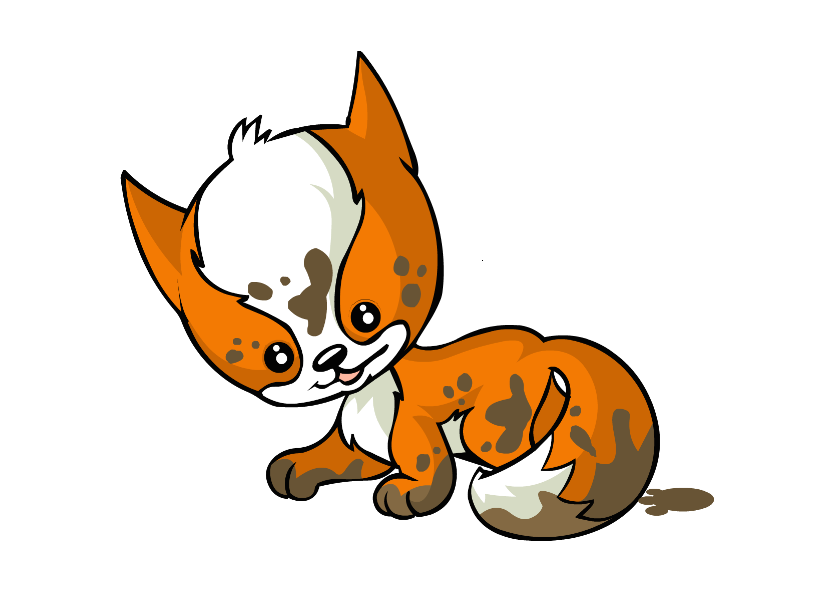
\includegraphics[scale=0.2]{serial_1/fox} & 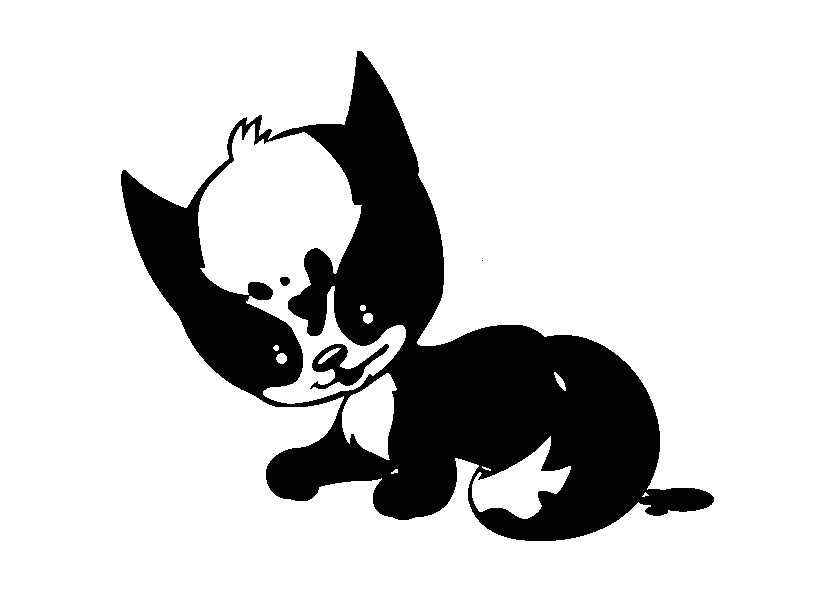
\includegraphics[scale=0.2]{serial_1/final} \\
        \small a) Original image & \small b) Approximated image
       \end{tabular}
       \caption{Image segmentation}
       \label{fig:seg}
\end{figure} 

Active contour without edge is proposed by Chan and Vese \cite{Chan2001}. This method find the approximated image by minimizing Mumford-Shah model:

\begin{equation}
E = \mu \text{ length}(C) 
+ \lambda\int_{\Omega}(f(x) - u(x))^2 dx
+ \int_{\Omega \\ C}|\nabla u(x)|^2 dx
\end{equation}
where
{\small
\begin{itemize}
    \item $\Omega$ denotes the image region
    \item $C$ denotes the contour of the region
    \item $f(x)$ is the intensity of image
    $\mu$ and $\lambda$ is constant
\end{itemize}
}

Generally, $u(x)$ is represented using level set function $\Phi$ on the domain of the image. Level set function is discretized to same size of the image. Final Chan-Vese model for level set function of minimal Mumford-Shah:

\begin{equation}
    \left\{ 
        \begin{aligned}
        & \frac{\partial \phi}{\partial t} = 
                \delta_{\epsilon} \left[
                \mu \text{ div} \left( \frac{\nabla \phi}{|\nabla \phi|} \right) - 
                \nu - 
                \lambda_1 (f-c_1)^2 +
                \lambda_2 (f-c_2)^2
                \right] \quad \text{ in } \Omega\\
        & \frac{\delta_{\epsilon}(\phi)}{|\nabla \phi|} 
            \frac{\partial \phi}{\partial \overrightarrow{n}}
            = 0
            \qquad \text{ on } \partial \Omega
        \end{aligned}
    \right.
\end{equation}
where

{\small
\begin{itemize}
    \item $c_1$  and $c_2$ is the mean intensity of the region inside and outside
    \item $\overrightarrow{n}$ is outward normal of the image boundary
    \item $\phi$ is the level set function
    \item $\delta_{\epsilon}(\phi) = \frac{\epsilon}{\pi (\epsilon^2 + \phi^2)}$ is Dirac function. Derivative of heaviside function $H_{\epsilon}(t)$
    \item $\nu$, $\eta$, $\lambda_1$ and $\lambda_2$ are constants.
\end{itemize}
}

For implementation, level set function is discretized to a matrix same size of the image. The convolution of $\phi$

\begin{equation}
    \begin{aligned}
            \frac{\partial \phi_{i, j}}{\partial t} = 
            \delta_{\epsilon}(\phi_{i,j}) \left[ \right.
                    & \left( A_{i,j}(\phi_{i+1, j} - \phi_{i,j})
                            - A_{i-1,j}(\phi_{i, j} - \phi_{i,j-1}) \right) \\
                    & + \left( B_{i, j}(\phi_{i, j+1} - \phi_{i, j}) - 
                             B_{i, j-1}(\phi_{i, j} - \phi_{i, j-1}) \right) \\
                    & - \nu - 
                        \lambda_1(f_{i,j} - c_1)^2 +
                        \lambda_2(f_{i, j} - c_2)^2 
                        \left. \right]
    \end{aligned}
    \label{eq:phi}
\end{equation}
where $A$ and $B$ are matrix same size with $\phi$.

\begin{equation}
    A_{i, j} = \frac{\mu}
                {\sqrt{\eta^2 
                       + (\nabla_x^+ \phi_{i, j} )^2
                       + (\nabla_y^0 \phi_{i, j} )^2 }
                }
    \label{eq:a}
\end{equation}

\begin{equation}
    B_{i, j} = \frac{\nu}
                    {\sqrt{\eta^2 
                            + (\nabla_x^0 \phi_{i, j} )^2
                            + (\nabla_y^+ \phi_{i, j} )^2 } 
                    }
    \label{eq:b}
\end{equation}
$\Delta \phi(i, j)$ denotes the difference of the level set function. There are forward, backward and central difference

\begin{equation}
    \begin{aligned}
        \nabla_x^- \phi(i, j) &= \phi_{i, j} - \phi_{i-1, j} \\
        \nabla_x^+ \phi(i, j) &= \phi_{i+1, j} - \phi_{i, j} \\
        \nabla_x^0 \phi(i, j) &= (\phi_{i+1, j} - \phi_{i-1, j} ) / 2
    \end{aligned}
\end{equation}

\chapter{Serial Algorithm}
\label{chap:serial}
Sample code is written by Getreuer \cite{Getreuer2012}. The algorithm is described in algorithm \ref{alg:chan-vese}.The sample results is shown in fig. \ref{fig:seg} and fig. \ref*{fig:prog}

\begin{algorithm}[hb]
    \DontPrintSemicolon
    \KwData{Image $I$}
    Initialize $\phi$ \;
    \For{ n = 1, .. }{
        Compute $c_1$ and $c_2$ \;
        \Begin(Compute $\phi^{n+1}$){
            Compute $A$ and $B$ \eqref{eq:a}, \eqref{eq:b}\;
            Compute $\frac{\partial \phi}{\partial t}$ \eqref{eq:phi}\;
            Compute $\phi^{n+1} = \phi^n + \frac{\partial \phi}{\partial t} \Delta t$
        }
        
        \textbf{if} $|\phi^{n+1} - \phi^n| < thres$ \textbf{then break} 
    }

    \caption{Numerical implementation}
    \label{alg:chan-vese}
\end{algorithm}


\begin{figure}[!htb]
    \centering
    \newcommand{\imgFoxProg}[1]{\includegraphics[trim=3cm 1cm 3cm 1cm, clip, scale=0.12]{serial_1/#1}}
    \imgFoxProg{1} \imgFoxProg{2} \imgFoxProg{3} \imgFoxProg{4} 
    \caption{Progress of segmentation}
    \label{fig:prog}
\end{figure}
